\documentclass[conference]{IEEEtran}
\usepackage{hyperref}
\usepackage{graphics} % Required for the inclusion of images
\usepackage{graphicx} % Required for the inclusion of images
\usepackage{caption}
\usepackage{amssymb}
\usepackage{amsmath}
\usepackage{subfigure}
\usepackage{pifont}
\usepackage{tikz}
\usepackage{pgfplots}
\usepackage{textcomp}
\usepackage{standalone}
\usepackage{import}
\usepackage{lipsum}
\usetikzlibrary{patterns}
\usetikzlibrary{calc}
\newcommand{\blue}[1]{\textcolor{blue}{#1}}
\newcommand{\red}[1]{\textcolor{red}{#1}}
\title{\LaTeX\, Gallery}

\author{
    \IEEEauthorblockN{Junyan Su}
    \IEEEauthorblockA{junyan.su@my.cityu.edu.hk}
}

\begin{document}
\maketitle

\begin{abstract}
    This is a small gallery of latex examples. I found some good figures/tables in the literature and reproduce them with latex. Every example corresponds to a standalone tex file in the folder submodules. A github repository is also available\footnote{\url{https://github.com/sujunyan/tex-gallery}}.
\end{abstract}


\begin{IEEEkeywords}
    \LaTeX , Figure, Table
\end{IEEEkeywords}

\section{Introduction}
% figure 2a/2b ----------------------
\lipsum
\begin{figure}[tb]
      \centering
      %\includegraphics[width=\linewidth]{submodules/2a/2a.pdf}
      %\documentclass[tikz]{standalone}
%\usepackage{pgfplots}
% the figures style are inspired by \url{https://www.nature.com/articles/nature14122/figures/12}.
% For the use of draw group line, refer to https://tex.stackexchange.com/questions/55554/how-can-i-mix-an-ybar-and-an-ybar-stacked-with-pgfplots
%\begin{document}



% figure a -------------------------------------------------------


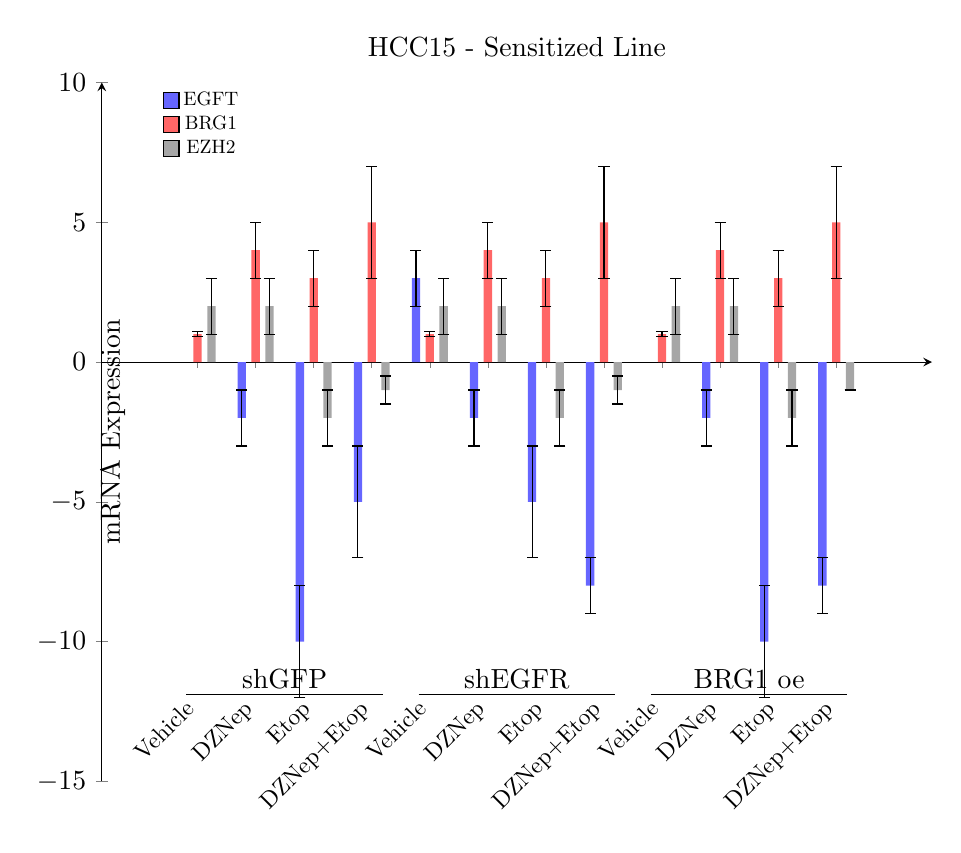
\begin{tikzpicture}
\newcounter{groupcnt}
% draw group line={<group column>}{<group value>}{<group label>}{<vertical offset>}{<line extension>}{<table name>}
\pgfplotsset{
    draw group line/.style n args={6}{
        after end axis/.append code={
            \setcounter{groupcnt}{0}
            \pgfplotstableforeachcolumnelement{#1}\of#6\as\cell{%
                \def\temp{#2}
                \ifx\temp\cell % if current row is in the group
                    \ifnum\thegroupcnt=0
                        \stepcounter{groupcnt}
                        \pgfplotstablegetelem{\pgfplotstablerow}{X}\of#6
                        \coordinate [yshift=#4] (startgroup) at (axis cs:\pgfplotsretval,0);
                    \else
                        \pgfplotstablegetelem{\pgfplotstablerow}{X}\of#6
                        \coordinate [yshift=#4] (endgroup) at (axis cs:\pgfplotsretval,0);
                    \fi
                \else % if we reach the end of current group
                    \ifnum\thegroupcnt=1
                        \setcounter{groupcnt}{0}
                        \draw [
                            shorten >=-#5,
                            shorten <=-#5
                        ] (startgroup) -- node [anchor=base, yshift=0.5ex] {#3} (endgroup);
                    \fi
                \fi
            }% end of for each column element
            \ifnum\thegroupcnt=1 % if we are at the end row
                        \setcounter{groupcnt}{0}
                        \draw [
                            shorten >=-#5,
                            shorten <=-#5
                        ] (startgroup) -- node [anchor=base, yshift=0.5ex] {#3} (endgroup);
            \fi
        }
    }
} % draw group line end -----------------

\pgfplotsset{my error bar/.style={
    error bars/.cd,y dir =both, y explicit,
  }
}

\pgfplotstableread{
X Gp  name EGFR EGFRerr BRG1 BRG1err EZH2 EZH2err
1 shGFP   Vehicle 0 0 1 0.1 2 1
2 shGFP   DZNep -2 1 4 1 2 1
3 shGFP   Etop -10 2 3 1 -2 1
4 shGFP   DZNep+Etop -5 2 5 2 -1 0.5
5 shEGFR  Vehicle 3 1 1 0.1 2 1
6 shEGFR  DZNep -2 1 4 1 2 1
7 shEGFR  Etop -5 2 3 1 -2 1
8 shEGFR  DZNep+Etop -8 1 5 2 -1 0.5
9  BRG1oe Vehicle 0 0 1 0.1 2 1
10 BRG1oe DZNep -2 1 4 1 2 1
11 BRG1oe Etop -10 2 3 1 -2 1
12 BRG1oe DZNep+Etop -8 1 5 2 -1 0.
}{\tabletwo}
\begin{axis}[
    width = \linewidth,
    title={HCC15 - Sensitized Line},
    ybar,
    bar width=3pt,
    axis x line = center, % change the default axis box.
    axis y line = left,
    enlarge x limits=0.15,
    ymin=-15, ymax=10,
    % legned related -------------
    legend image code/.code={
        \draw [#1] (0cm,-0.1cm) rectangle (0.2cm,0.1cm);
    },
    legend style={
        at={(0.18,1)},
        nodes={scale=0.7},
        draw = none     % without box
    },
    ylabel={mRNA Expression},
    % xtick related 
    xtick=data,
    xticklabels from table={\tabletwo}{name},
    xticklabel style={
        rotate=45,xshift=-85,yshift=-85,
        anchor=mid east,
        scale=0.85,
    },
    ylabel style={at={(axis description cs:0.04,0.5)}},
    draw group line={Gp}{shGFP}{shGFP}{-120}{4pt}{\tabletwo},
    draw group line={Gp}{shEGFR}{shEGFR}{-120}{4pt}{\tabletwo},
    draw group line={Gp}{BRG1oe}{BRG1 oe}{-120}{4pt}{\tabletwo},
    ] % end of options of axis environment

% the "!" denotes the intensity
\addplot [draw=none, fill=blue!60,my error bar] table [y=EGFR,y error=EGFRerr] {\tabletwo};
\addplot [draw=none, fill=red!60,my error bar] table [y=BRG1,y error=BRG1err] {\tabletwo};
\addplot [draw=none, fill=gray!70,my error bar] table [y=EZH2,y error=EZH2err] {\tabletwo};

\legend{EGFT,BRG1,EZH2}

\end{axis}
\end{tikzpicture}

%\end{document}
    \caption{sub-figure from Extended Data Figure 8 in~\cite{2}.}
\end{figure}

\lipsum[1]
\begin{figure*}[tb]
  \centering
  %\documentclass[tikz]{standalone}
%\usepackage{pgfplots}
%\usetikzlibrary{calc}

% the figures style are inspired by \url{https://www.nature.com/articles/nature14122/figures/12}.
% For the use of draw group line, refer to https://tex.stackexchange.com/questions/55554/how-can-i-mix-an-ybar-and-an-ybar-stacked-with-pgfplots
%\begin{document}
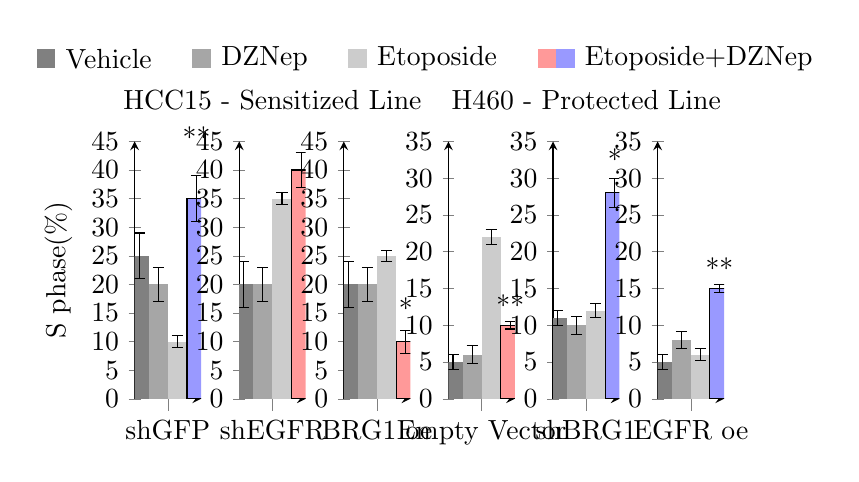
\begin{tikzpicture}
\pgfplotsset{my error bar/.style={error bars/.cd,y dir =both, y explicit}}
\pgfplotsset{
    subplotStyle/.style n args ={1}{
        axis x line = bottom, % change the default axis box.
        axis y line = left,
        width = 0.2\linewidth ,
        height = 0.4\linewidth ,
        ybar=0,
        bar width = 0.02\linewidth ,
        ytick={0,5,...,45},
        ymin=0,ymax=45,
        nodes={scale=1},
        xtick=data,
    }
}
\newcommand{\subplotxoffset}{.04\linewidth}
% plot1 ---------------------------
\newcommand{\subplotName}{shGFP}
\begin{axis}[
    name=plot1,
    ylabel=S phase(\%),
    symbolic x coords={\subplotName},
    subplotStyle={45},
]

\addplot [draw=none,fill=gray!100,my error bar] coordinates {(\subplotName,25)+-(0,4)};
\addplot [draw=none,fill=gray!70,my error bar] coordinates {(\subplotName,20)+-(0,3)};
\addplot [draw=none,fill=gray!40,my error bar] coordinates {(\subplotName,10)+-(0,1)};
\addplot [
    nodes near coords={**},
    nodes near coords style = {
       yshift=15pt,xshift=0pt,
    },
    fill=blue!40,
    my error bar,
    ] coordinates {(\subplotName,35)+-(0,4)};
\end{axis}

% plot2 ----------------------------
\renewcommand{\subplotName}{shEGFR}
\begin{axis}[
    name=plot2,
    at = {($(plot1.east)+(\subplotxoffset,0)$)},
    anchor=west,
    %enlargelimits=0.05,
    symbolic x coords={\subplotName},
    subplotStyle={45},
]
\addplot [draw=none,fill=gray!100,my error bar] coordinates {(\subplotName,20)+-(0,4)};
\addplot [draw=none,fill=gray!70,my error bar] coordinates {(\subplotName,20)+-(0,3)};
\addplot [draw=none,fill=gray!40,my error bar] coordinates {(\subplotName,35)+-(0,1)};
\addplot [fill=red!40,my error bar] coordinates {(\subplotName,40)+-(0,3)};
\end{axis}

% plot3 --------------------------------
\renewcommand{\subplotName}{BRG1 oe}
\begin{axis}[
    name=plot3,
    at = {($(plot2.east)+(\subplotxoffset,0)$)},
    anchor=west,
    %enlargelimits=0.05,
    symbolic x coords={\subplotName},
    subplotStyle={45},
]
\addplot [draw=none,fill=gray!100,my error bar] coordinates {(\subplotName,20)+-(0,4)};
\addplot [draw=none,fill=gray!70,my error bar] coordinates {(\subplotName,20)+-(0,3)};
\addplot [draw=none,fill=gray!40,my error bar] coordinates {(\subplotName,25)+-(0,1)};
\addplot [
    nodes near coords={*},
    nodes near coords style = {
       yshift=5pt,xshift=0pt,
    },
    fill=red!40,my error bar
    ] coordinates {(\subplotName,10)+-(0,2)};
\end{axis}

\renewcommand{\subplotName}{Empty Vector}
\begin{axis}[
    name=plot4,
    at = {($(plot3.east)+(\subplotxoffset,0)$)},
    anchor=west,
    %enlargelimits=0.05,
    symbolic x coords={\subplotName},
    subplotStyle={45},
    ymax=35,
]
\addplot [draw=none,fill=gray!100,my error bar] coordinates {(\subplotName,5)+-(0,1)};
\addplot [draw=none,fill=gray!70,my error bar] coordinates {(\subplotName,6)+-(0,1.2)};
\addplot [draw=none,fill=gray!40,my error bar] coordinates {(\subplotName,22)+-(0,1)};
\addplot [
    nodes near coords={**},
    nodes near coords style = {
       yshift=0pt,xshift=0pt,
    },
    fill=red!40,my error bar] 
    coordinates {(\subplotName,10)+-(0,0.5)};
\end{axis}

% plot5 -----------------------------------
\renewcommand{\subplotName}{shBRG1}
\begin{axis}[
    name=plot5,
    at = {($(plot4.east)+(\subplotxoffset,0)$)},
    anchor=west,
    %enlargelimits=0.05,
    symbolic x coords={\subplotName},
    subplotStyle={45},
    ymax=35,
]
\addplot [draw=none,fill=gray!100,my error bar] coordinates {(\subplotName,11)+-(0,1)};
\addplot [draw=none,fill=gray!70,my error bar] coordinates {(\subplotName,10)+-(0,1.2)};
\addplot [draw=none,fill=gray!40,my error bar] coordinates {(\subplotName,12)+-(0,1)};
\addplot [
    nodes near coords={*},
    nodes near coords style = {
       yshift=5pt,xshift=0pt,
    },
    fill=blue!40,my error bar
    ] coordinates {(\subplotName,28)+-(0,2)};
\end{axis}

% plot6 -----------------------------------
\renewcommand{\subplotName}{EGFR oe}
\begin{axis}[
    name=plot6,
    at = {($(plot5.east)+(\subplotxoffset,0)$)},
    anchor=west,
    %enlargelimits=0.05,
    symbolic x coords={\subplotName},
    subplotStyle={45},
    ymax=35,
    %% the legends to be placed outside 
    legend image code/.code={
        \draw [#1] (0cm,-0.1cm) rectangle (0.2cm,0.1cm);
    },
    legend style={
        legend columns=-1,
        draw=none,
        fill=none,
    },
    legend entries={Vehicle,DZNep,Etoposide,Etoposide+DZNep},
    legend to name=commonLegendb,
]
\addplot [draw=none,fill=gray!100,my error bar] coordinates {(\subplotName,5)+-(0,1)};
\addplot [draw=none,fill=gray!70,my error bar] coordinates {(\subplotName,8)+-(0,1.2)};
\addplot [draw=none,fill=gray!40,my error bar] coordinates {(\subplotName,6)+-(0,0.8)};
\addplot [
    nodes near coords={**},
    nodes near coords style = {
       yshift=0pt,xshift=0pt,
    },
    fill=blue!40,my error bar
    ] 
    coordinates {(\subplotName,15)+-(0,0.5)};
\end{axis}
%% end of the plots ----------------------

% plot the title for the two groups
\node [scale=1] (title1) at ($(plot1.north)!0.5!(plot3.north)+(0,15pt)$) {HCC15 - Sensitized Line};
\node [scale=1] (title2) at ($(plot4.north)!0.5!(plot6.north)+(0,15pt)$) {H460 - Protected Line};

% self draw the legend ---------------
\node [matrix,fill=none,draw=none] (mylegendnode) at ($(title1.north)!0.5!(title2.north)+(0,8pt)$)
{
\node [fill=gray!100,shape=rectangle,label=right:Vehicle]{}; &[4mm]
\node [fill=gray!70,shape=rectangle,label=right:DZNep]{}; &[4mm]
\node [fill=gray!40,shape=rectangle,label=right:Etoposide]{}; &[4mm]
\node [fill=red!40,shape=rectangle]{}; &
\node [fill=blue!40,shape=rectangle,label=right:Etoposide+DZNep]{}; \\
};

% draw legend with pgfplot function (Not work well)--------------
%\node [scale=0.8] (mylegendnode) at ($(title1.north)!0.5!(title2.north)+(0,8pt)$) {\pgfplotslegendfromname{commonLegendb}};

\end{tikzpicture}

%\end{document}
  \caption{sub-figure from Extended Data Figure 8 in~\cite{2}.}
\end{figure*}

\lipsum
\lipsum[1]
% figure 1 ------------------------------------------
\begin{figure*}[htb]
    \begin{center}
        %\includegraphics[width=.8\linewidth]{submodules/1/1.pdf}
        % style from fig.11 in https://ieeexplore.ieee.org/abstract/document/9031358
\begin{tikzpicture}
\pgfplotstableread{submodules/1/datafile1.csv}{\datatable}
\begin{axis}[
  xlabel={Computation time passed~[minutes]},
  ylabel={bits per channel use},
  ylabel style={at={(axis description cs:0.03,0.5)}},
  xmin= 0, xmax= 120, ymin= 0,
  legend style = {
      legend pos=south east,
      legend columns = {2},
      nodes={scale=0.8}, % make the legend box smaller
      %font = {\tiny},
  },
  grid = major,
  grid style=dashed,
  mark repeat={8},
  width = \linewidth,
  height = 0.5\linewidth,
  mark options={solid},
  %% extra label for information rate
  every axis/.append style={
      extra description/.code={
          \node[scale=0.5] at (0.07,0.93) {Information Rate};
          \node[scale=0.5] at (0.93,0.93) {Information Rate};
      },
  },
] % end of axis setting

  %1
  \addplot[red,mark=o,dashed] table [x index=0, y index=1] {\datatable};
  \addlegendentry{EM-type algorithm~[13] with 4-state FSMC}

  %2
  \addplot[dashed,mark=o] table [x index=0, y index=2] {\datatable};
  \addlegendentry{EM-type algorithm~[13] with 16-state FSMC}

  %3
  \addplot[blue,mark=diamond] table [x index=0, y index=3] {\datatable};
  \addlegendentry{Algorithm~11 with 1-qubit QSC}

  %4
  \addplot[red,mark=+] table [x index=0, y index=4] {\datatable};
  \addlegendentry{Algorithm~11 with 4-state FSMC}

  %5
  \addplot[mark=+] table [x index=0, y index=5] {\datatable};
  \addlegendentry{Algorithm~11 with 16-state FSMC}

  %6
  \addplot[red,mark=diamond] table [x index=0, y index=6] {\datatable};
  \addlegendentry{Algorithm~11 with 2-qubit QSC}

  %7
  \addplot[dashed] table [x index=0, y index=7] {\datatable};
  \addlegendentry{Estimated Information Rate~(Alg.~9)}

\end{axis}
\end{tikzpicture}
    \end{center} 
    \caption{This is fig.11 from~\cite{1}}
\end{figure*}

% figure 3a/3b -----------------------------
\lipsum
\begin{figure*}[htb]
    \begin{center}
        \subfigure[A subcaption]{
            %\includestandalone[width=.48\linewidth]{submodules/3a/3a}
            \includegraphics[width=0.48\linewidth]{submodules/3a/3a.pdf}
        }
        \subfigure[A subcaption]{
            \includegraphics[width=0.48\linewidth]{submodules/3b/3b.pdf}
            %\includestandalone[width=.48\linewidth]{submodules/3b/3b}
        }
    \end{center} 
    \caption{(A figure across two columns)}
\end{figure*}

% usage \includeSubmodule{name}{additional caption}{*?}
\newcommand{\includeSubmodule}[3]{
    \begin{figure#3}[!htb]
        \begin{center}
            \includegraphics[width=\linewidth]{submodules/#1/#1.pdf}
        \end{center} 
        \caption{#2}
    \end{figure#3}
}

\lipsum[1]
\includeSubmodule{4}{pcode example}{}
\lipsum[1]
\includeSubmodule{6}{table example 02}{*}
\lipsum[1]

\newcommand{\xmark}{\ding{55}}%package pifont
\begin{table}[h]
  \centering
  \begin{tabular}{|c|c|c|c|}
    \hline
    Paper & Route Planning & Speed Planning & Hard Deadline \\  \hline
    [37] & \checkmark & \xmark & \xmark \\ \hline
    [16] & \xmark & \checkmark & \xmark \\ \hline
    [17] & \xmark & \checkmark &  \checkmark \\ \hline
    This work & \checkmark&\checkmark & \checkmark\\ \hline
  \end{tabular}
  \caption{Table~II from~\cite{deng2017energy}}
\end{table}
\lipsum
\includeSubmodule{5}{table example 01}{*}
\lipsum

\bibliographystyle{unsrt}
\bibliography{ref}
\end{document}